\oz{} can be used to model an entity with fixed operations, but some time we need to model entities with unfixed operations. We need a Dynamic version of \oz{}. To solve this problem we introduce the concepts of \findex{Operation schema overloading} and \findex{Unfixed operation schema}.
\subsubsection{Operation schema overloading}
Imagine that our vending machine $VM$ is a mobile vending machine and that it is connected by a wireless link $talk$ to a shop $Shop1$. On signal fading $Shop1$ decides to send the link $talk$ to another shop $Shop2$ through the link $switch$ as shown in \refFig{fig_oz_mobile_vending_machine_and_shops}. \oz{} can be used to model the shop. But, the operation $switch$ has a dual nature. It plays the sender role in $Shop1$, and the receiver role in $Shop2$.
 In \oz{} to deal with this duality nature we introduce the concept of \findex{Operation schema overloading}. As in some programming languages, method overloading is the ability to create multiple methods of the same name with different implementations. That is, the operation $switch$ has two different specifications ,i.e. two operation schemas with the same name as shown in \refFig{fig_oz_overloaded_operation_shop}, the first for sending the link $talk$ and the second for receiving it.
When a $VM$ talks to a shop it sends its $id$ and a message $m$. The shop will store them in its state variables $vmID$ and $m$ as shown in \refFig{fig_oz_overloaded_operation_shop} in the operation schema $talk$.
\begin{figure}[H]%
\centering
\subcaptionbox{Before switch}{\fbox{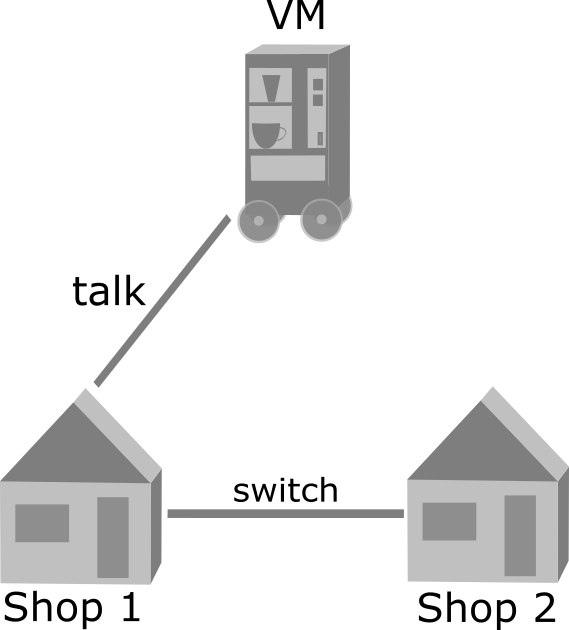
\includegraphics[width=0.45\textwidth]{./images/preliminaries/oz/oz_mobile_vending_machine_and_shops1.png}}}%
\hfill
\subcaptionbox{After switch}{\fbox{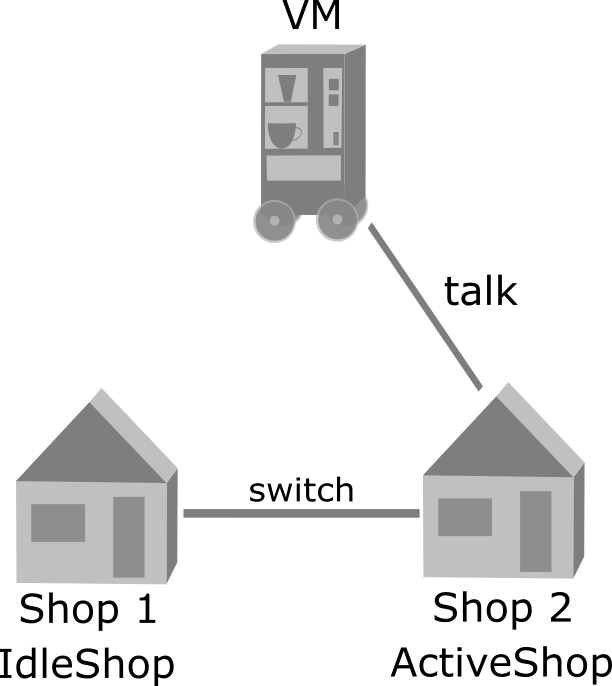
\includegraphics[width=0.45\textwidth]{./images/preliminaries/oz/oz_mobile_vending_machine_and_shops2.png}}}%
\caption{Mobile vending machine and shops}
\label{fig_oz_mobile_vending_machine_and_shops}%
\end{figure}

\begin{figure}[H]
\centering
\begin{class}{Shop(id: \integer)}
\\
\begin{state}
m, vmId, self: \integer
\end{state} 
\\
\begin{init}
\\self = id
\end{init} 
\\
\begin{op}{switch}
x!: chan[\integer \times \integer]
\ST
x! = talk
\end{op}
\\
\begin{op}{switch}
\\x?: chan[\integer \times \integer]
\ST
x? = talk
\end{op}
\\
\begin{op}{talk}
\Delta (m,vmId)
\\y?: \integer
\\z?: \integer
\ST
y? = m'
\\z? = vmId'
\end{op}
\end{class}
\caption{$Shop$ class: \textit{operation schema overloading.}}
\label{fig_oz_overloaded_operation_shop}
\end{figure}



\subsubsection{Unfixed operation schema}
Let us have another look at \refFig{fig_oz_mobile_vending_machine_and_shops}. We can notice that before switching $Shop1$ was able to invoke the operation $talk$, but after switching this is not possible, since the link $talk$ moved to $Shop2$. In \oz{} words:
\begin{itemize}
\item Before switching:
	\begin{itemize}
	\item $Shop1$: has the operation schema $talk$
	\item $Shop2$: doesn't have the operation schema $talk$
	\end{itemize}
\item By switching: $Shop1$ sends its operation schema $talk$ to $Shop2$.
\item After switching:
	\begin{itemize}
	\item $Shop1$: doesn't have the operation schema $talk$
	\item $Shop2$: has the operation schema $talk$
	\end{itemize}
\end{itemize}
That means, when we model the $talk$ operation in \oz{} we need to consider the following problems: 

\begin{itemize}
\item In \oz{}, it is not possible to send an \underline{operation} from $Shop1$ to $Shop2$.\\
\textbf{Solution:} By calling $talk$ an unfixed operation, and By using a state variable $t$ to store the name of the unfixed operation as shown in \refFig{fig_oz_unfixed_operation_schema_shop}.\\
By switching:
\begin{itemize}
\item $Shop1$ is the sender, so it sets its state variable $t$ to $nil$, which means the operation $talk$ is no more available on $Shop1$.
\item $Shop2$ is the receiver, so it sets its state variable $t$ to the value received from $Shop1$, .i.e., $talk$, which means: the operation $talk$ is now available on $Shop2$.
\end{itemize}
\item In \oz{}, it is not possible to send an \underline{operation schema} from $Shop1$ to $Shop2$.\\
\textbf{Solution:} Unfixed operation schema. To make the $talk$ operation schema in \refFig{fig_oz_overloaded_operation_shop} an unfixed operation schema, .i.e., a conditional operation schema as shown in \refFig{fig_oz_unfixed_operation_schema_shop}, it says: if $t = talk$ then this schema is the $talk$ operation schema, otherwise this schema doesn't exists.

\end{itemize}


\begin{figure}[H]
\centering
\begin{class}{Shop(id: \integer)}
\\
\begin{state}
m, vmId, self: \integer
\\t: chan[\integer \times \integer]
\end{state} 
\\
\begin{init}
\\self = id
\end{init} 
\\
\begin{op}{switch}
x!:  chan[\integer \times \integer]
\ST
x! = t
\\t' = nil
\end{op}
\\
\begin{op}{switch}
\Delta (t)
\\x?:  chan[\integer \times \integer]
\ST
x? = t'
\end{op}
\\
\begin{op}{\text{if } t = talk \text{ then } talk \text{ else } undefined}
\Delta (m,vmId)
\\y?: \integer
\\z?: \integer
\ST
y? = m'
\\z? = vmId'
\end{op}
\end{class}
\caption{$VM$ class: \textit{unfixed operation schema.}}
\label{fig_oz_unfixed_operation_schema_shop}
\end{figure}


\subsubsection{Restriction}
In this work when we use \oz{} to model an operation, we restrict our self to use only one type of parameters in the operation schema. Either input or output. This can be noticed in the operation schema $talk$ in:
\begin{itemize}
\item In \refFig{oz_vm_reference_name} all the parameters of the operation schema $talk$ are output paramaters.
\item In \refFig{fig_oz_unfixed_operation_schema_shop}  all the parameters of the operation schema $talk$ are input paramaters.
\end{itemize}
\textbf{Question:} why this restriction?\\
\textbf{Answer:} because a channel in \picalc{} is unidirectional pro reaction. In the next chapter we will map the \oz{} class constructs to  \picalc{} constructs, so we will map an \oz{} operation to an \picalc{} name , .i.e., channel. In \picalc{} a processes can send or receive over a channel pro reaction, but not the both together.